\chapter{Arhitectura soluţiei}

\section{Prezentare generală}
Alegria a fost conceputa ca o platforma de dezvoltare rapida, bazata pe modele. Prin folosirea unor metode de programare vizuala, cu blocuri refolosibile in mai multe aplicaţii diferite, utilizatorul poate sa îşi concentreze resursele asupra soluţiei finale, abstractizând detaliile implementării. 
Aplicaţia a fost construita pe baza unei arhitecturi modulare, cu module cat mai puţin cuplate, care sa permită modificări rapide si testarea modulelor individual. Urmărind aceasta gândire modulare, au fost s-au identificat 4 componente esenţiale: 
\begin{itemize}
	\item \textbf{Baza de date} Asigură stocarea datelor, dar si a entităţilor existente in aplicaţie;
	\item \textbf{Interfaţa web pentru management} O interfaţă uşor de utilizat care sa permită  utilizatorului să manipuleze canale, diagrame, blocuri de procesare, dar si alţi utilizatori
	\item \textbf{API-ul pentru date} Un API specializat pentru adăugare de date, achiziţionarea datelor, dar si sa permită altor dispozitive sa fie notificate de fiecare data când apar date noi.
	\item \textbf{Elemente de procesare} Asigură procesarea datelor, atât in cadrul blocurilor de procesare, dar si in cadrul diagramelor funcţionale.
\end{itemize}
\begin{figure}
	\centering
	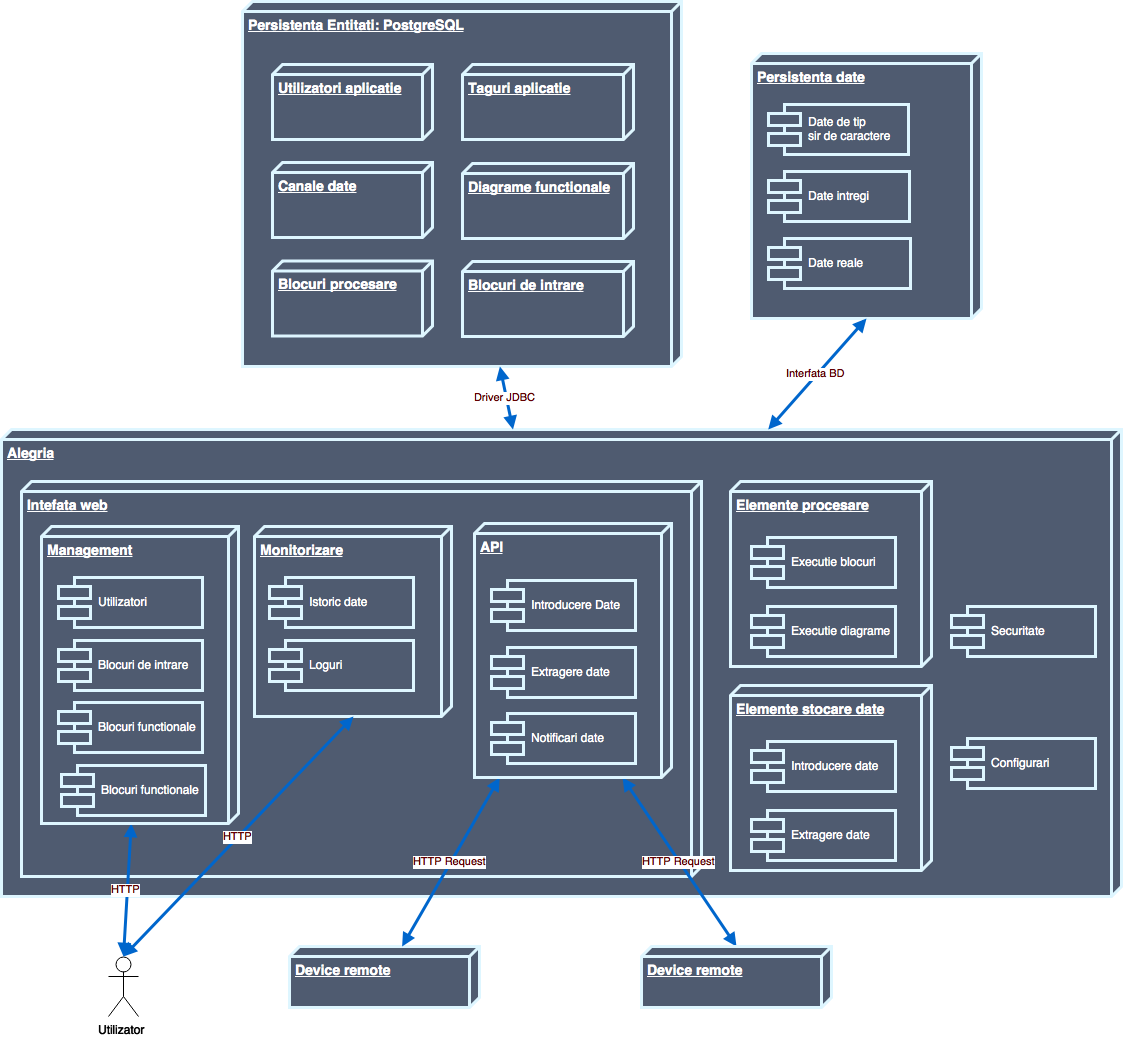
\includegraphics[width=1.3\textwidth, center]{arhitecturaGenerala}
	\caption{Arhitectura generala a aplicaţiei}
	\label{fig:arhitecture}
\end{figure}

In vederea implementării sistemului s-au identificat următoarele elemente componente esenţiale, componente ce reprezinta elementele constructive a sistemului. Acestea, au reprezentare atât in baza de date, ca entităţi, cat si in aplicaţia Java, ca clase. Identificarea acestor elemente s-a făcut pe baza analizei cazurilor de utilizare a produsului, in care s-au investigat metodele prin actorii interacţionează cu sistemul.
\begin{itemize}
\label{list:entities}
\item \textbf{Canalul de date:} reprezinta elementul de baza a sistemului, care asigura recepţia, persistenta si emiterea de date. Datele dintr-un canal trebuie sa respecte un format prestabilit la crearea canalului. Pentru transformarea datelor in formatul stabilit, se poate introduce un bloc de pre-procesarea care transforma datele din un format brut in formatul standard.
\item \textbf{Blocul de intrare:} elementul de intrare, alcătuit din mai multe canale de date. Blocurile de intrare permit gruparea mai multor canale de date într-o structura unica.   
\item \textbf{Blocul de procesare:} elementul dinamic al aplicaţiei, ce aplica transformări asupra datelor. Un bloc de procesare primeşte ca intrări mai multe canale de date, si are la ieşire un alt canal de date. Utilizatorul poate folosi blocuri standard, existente in sistem, sau poate implementa blocuri noi direct in interfaţa programului.
\item \textbf{Diagrama funcţie bloc(FBD):}  foloseşte blocuri de intrare, canale de date si blocuri de procesare pentru a descrie o funcţie complexa intre intrări si o ieşire. Aceste diagrame folosesc la date aflate pe canale de date, care sunt trimise către blocuri de procesare si, la final se obţine un singur rezultat care este salvat pe un canal de date.
\end{itemize}

\subsection{Baza de date}

Fiind vorba despre o aplicaţie puternic bazata pe date, aceasta are nevoie de un nivel de persistenta de înaltă performaţă. 
Urmărind arhitectura propusă din \cref{fig:arhitecture}, putem identifica doua cazuri de utilizare pentru baza de date: 
\begin{itemize}
	\item Stocarea modelului entităţilor: fiecare entitate descrisa in lista de mai sus trebuie stocata in baza de date într-o structura relaţională. Entităţile sunt puternic interconectate, iar o baza de date relaţională, de tip SQL este recomandata in acest caz. 
	Din punct de vedere a dimensiunii setului de date, chiar si in aplicaţiile de mare complexitate, este vorba despre doar câteva milioane de înregistrări, factorul care face acest număr să crească fiind conectarea a tot mai mult dispozitive, ce duce la din ce in ce mai multe canale de date. Astfel, stocarea entităţilor nu va aduce probleme de performaţă. 
	\item Stocarea datelor: in baza de date vor fi stocate atât datele primite pe fiecare canal asociat unui bloc de intrare, cat si datele procesate de diagrame. Aceste date au un puternic caracter istoric, reprezentând o serie de timp, in care se retine, pentru fiecare punct de date, valoarea la un anumit moment. Problema stocării acestor date este una mai complicata, datorita necesităţii unei puternice scalari a bazei de date. Această problemă reprezinta un caz de utilizare pentru o baza de date NoSQL, sau chiar o baza de date specializata in stocarea seriilor de timp \autocite{openTSDB}.  
\end{itemize}

\subsection{Aplicaţia Java}
Legătura dintre baza de date si utilizatorii finali se face prin intermediul unei aplicaţii Java complexe, care este obiectul acestui proiect. Aplicaţia conţine toată logica platformei, de la operaţii asupra entităţilor din baza de date, la adăugarea, si extragerea datelor, cat si pentru procesarea datelor. 
Separarea modulelor s-a făcut pe baza scopului acestora:
\begin{itemize}
	\item \textbf{Administrare}: pentru administrarea entităţilor din baza de date. Aceste module permit operaţii de căutare si afişare, dar si de creere, editare si ştergere a utilizatorilor, a blocurilor de intrare si funcţionale precum si a diagramelor. Fiecare dispune de o interfaţă HTML5 in care moderna. 
	\item \textbf{Monitorizare}: permit monitorizarea execuţiei aplicaţiei, de la vizualizat loguri pentru a diagnostica probleme, la realizarea de grafice a datelor pe anumite canale. Tot aici este disponibila si funcţia de a exporta date in formate uzuale, ca CSV sau fişiere Microsoft Excel.
	\item \textbf{API}: aplicaţia dispune si de un API pentru a fi folosita programatic de către alte aplicaţii externe. Acesta poate fi considerat ca fiind format din doua componente: serviciile pentru administrarea entităţilor, si cele pentru adăugarea si extragerea datelor.
	\item \textbf{Elemente de procesare}: împărţite in doua subcategorii: cele pentru procesarea blocurilor de intrare si de procesare, si cele pentru procesarea diagramelor.
	\item \textbf{Elemente stocare date}: permit interfaţarea cu sursele de date. Acestea asigura servicii de introducere si extragere a datelor, printr-o interfaţă abstracta, care nu tine cont de modul in care baza de date este implementata.
	\item \textbf{Alte module}: asigura, printre altele securitatea aplicaţiei.
\end{itemize}

\section{Entităţi}
\subsection{Punctul de date}

Punctul de date reprezinta elementul constructiv al sistemul, care este obiectul procesării, stocării si distribuţiei este punctul de date. 
Sistemul accepta intern date in formatele: 
\begin{wrapfigure}{r}{0.38\textwidth}
	\centering
	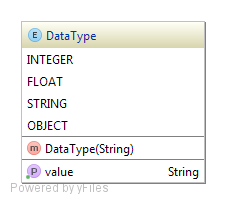
\includegraphics[width=0.38\textwidth]{dataType}
	\caption{Tipurile de date acceptate in sistem}
\end{wrapfigure}
\begin{itemize}
	\item \textbf{Întreg}: numere de la $-2^{63}$ la $2^{63} -1$, fără virgula, foloseşte \textit{Long} pentru reprezentare interna;
	\item \textbf{Real}: numere cu virgula, având dubla precizie, reprezentate cu 64-bit conform standardului \autocite{4610935} IEEE 754  foloseşte \textit{Double} pentru reprezentare interna;
	\item \textbf{Sir de caractere}: Un sir de fără limite a lungimii, care trebuie formatat conform \autocite{rfc4627}. 
	\item \textbf{Obiect}: Un obiect Java serializat in text. Intern, asemănător cu tipul de date String. 
\end{itemize}

\begin{figure}[h]
	\centering
	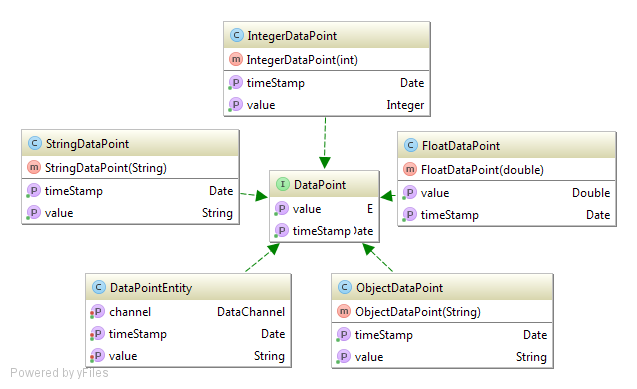
\includegraphics[width=1.1\textwidth, center]{dataPoint}
	\caption{Clasele care implementează interfaţa DataPoint}
\end{figure}

\subsection{Canalul de date}

Canalul de date este entitatea care asigura "curgerea" datelor prin sistem. Orice punct de date din sistem aparţine unui canal, acest lucru fiind realizat drept constrângere atât la nivelul aplicaţiei, cat si la nivelul bazei de date.
\begin{figure}[h]
	\centering
	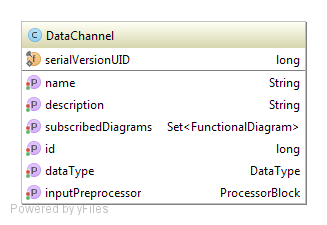
\includegraphics[width=0.55\textwidth]{dataChannel}
	\caption{Clasa DataChannel}
\end{figure}
Canalul este si mijlocul prin care utilizatorul interacţionează cu punctele de date. Pentru a adaugă date noi, un sistem le ataşează unui canal, diagramele folosesc canale atât pentru date de intrare cat si pentru date de ieşire, iar utilizatorii externi pot extrage datele de pe un canal.

\subsection{Blocul de intrare}

\begin{figure}[h]
	\centering
	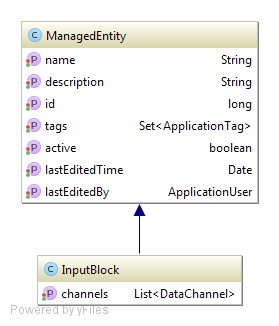
\includegraphics[width=0.55\textwidth]{inputBlock}
	\caption{Clasa InputBlock}
\end{figure}
\subsection{Primirea datelor}
Primirea datelor se face prin intermediul unei interfeţe de transfer a stării (REST). Mai multe formate sunt incluse pentru integrarea mai uşoară cu sisteme deja existente. Astfel, au fost implementate mai multe procesoare care primesc date atât într-un format special, cat si in formate standard in industrie.
Astfel, doua modalităţi de trimitere a datelor exista in sistem:
\begin{sidewaysfigure}
	\centering
	\includegraphics[width=\textwidth]{introducereDate}
	\caption{Diagrama de secvente pentru intorducerea de noi date}
	\label{fig:intrareDate}
\end{sidewaysfigure}
\begin{itemize}
	\item Trimitere către un singur canal, un singur punct odată: pe baza serviciului\\ \textit{/api/put/{inputId}/{channelId}/{data}}. Acest serviciu adaugă un singur punct in baza de date, la momentul curent. Folosit pentru sisteme care trimit date rar, si nu trebuie sa se tina cont de data locala de pe device-ul care a trimis punctul de date.
	\item In formatul standard folosit de openTDSB in care au fost introduse următoarele modificări care păstrează totuşi compatibilitatea: metricile reprezinta numele canalului, iar tag-urile sunt opţionale. Se acceptat atât formatul in care într-o cerere se afla un singur punct, cat si formatul cu o lista de puncte. Canalele dintr-o cere multidimensionala nu trebuie sa facă parte din acelaşi bloc de intrare. Acest mod de introducere a datelor este sugerat pentru sistemele care folosesc mai multe canale de date si care trimit seturi de date mai mari printr-o singura cerere. Spre exemplu, un dispozitiv poate trimite date de pe mai multi senzori, si poate stoca local mai multe măsurători pe acelaşi senzor pentru a trimite toate datele odată.
\end{itemize}
Odată primite, noile puncte de date trec prin procesul descris in \cref{fig:intrareDate}:
\begin{enumerate}
	\item Se interoghează baza de date pentru detalii privind canaul ce tocmai a primit date
\end{enumerate}



